\documentclass[conference]{IEEEtran}
\usepackage{times}
\usepackage{algorithm}
\usepackage{algpseudocode}
\usepackage{subfigure}
\usepackage{graphicx}
\usepackage{subfloat}
\usepackage{float}
\usepackage{mathtools}% http://ctan.org/pkg/mathtools
\usepackage{amsmath,empheq}
\usepackage{amssymb}
\usepackage{latexsym}
%\usepackage{bbm}

\usepackage[numbers]{natbib}
\usepackage{multicol}
\usepackage[bookmarks=true]{hyperref}
\usepackage[usenames,dvipsnames]{color}
\usepackage{tikz}
\usepackage{pgfplots}

% -- Comment commands --
\newcommand{\stnote}[1]{\textcolor{Blue}{\textbf{ST: #1}}}
\newcommand{\dnote}[1]{\textcolor{Green}{\textbf{D: #1}}}
\newcommand{\enote}[1]{\textcolor{Red}{\textbf{E: #1}}}
\newcommand{\gnote}[1]{\textcolor{Purple}{\textbf{G: #1}}}

% -- Misc. new commands --
\newcommand{\argmax}{\operatornamewithlimits{argmax}}

\pdfinfo{
% We'll talk about authorship when we're all together
   /Author (David Abel \& Gabriel Barth-Maron, James MacGlashan, Stefanie Tellex)
   /Title  (Toward Affordance-Aware Planning)
   /CreationDate (D:20101201120000)
   /Subject (Planning, Affordances, Sequential Decision Making)
   /Keywords (Planning, Affordance, MDP, Learning)
}

\begin{document}

% paper title
\title{Affordance-Aware Planning}

% Author info:
\author{\authorblockN{David Abel \& Gabriel Barth-Maron, James MacGlashan, Stefanie Tellex}
\authorblockA{Computer Science Department, Brown University \\
\texttt{\{dabel,gabrielbm,jmacglashan,stefie10\}@cs.brown.edu}}}

\maketitle

\begin{abstract}
Planning algorithms for non-deterministic domains are often
intractable in large state spaces due to the well-known curse of
dimensionality. Existing approaches to planning in large stochastic
state spaces fail to prevent autonomous agents from considering many
actions that are obviously irrelevant to a human solving the same
task. To reduce the size of the state/action space without sacrificing
optimality, we formalize the notion of {\em affordances} as
goal-oriented knowledge added to an Object Oriented Markov Decision
Process (OO-MDP).  Affordances prune actions based on the current
state and the robot's goal, reducing the number of state-action pairs
the planner must evaluate in order to synthesize a near optimal
policy. We show that an agent can learn affordances through
unsupervised\dnote{Do you agree that this is unsupervised?} experience, and that learned affordances can equal or
surpass the performance of those provided by experts. We demonstrate
our approach in the state-rich Minecraft domain, showing significant
increases in speed and reductions in state-space exploration during
planning, with minimal loss in quality of the synthesized policy.
Additionally, we employ affordance-aware planning on a Baxter robot,
demonstrating it is able to assist a person performing a collaborative
cooking task.

\end{abstract}

\IEEEpeerreviewmaketitle

% ====== Section: Introduction ======
\section{Introduction}
\label{sec:introduction}

Robots operating in unstructured, stochastic environments such as a
factory floor or a kitchen face a difficult planning problem due to
the large state space and inherent
uncertainty~\citep{bollini12,knepper13}.  Robotic planning tasks are
classically formalized as a stochastic sequential decision making
problem, modeled as a Markov Decision Process (MDP). In these
problems, the agent must find a mapping from states to actions for
some subset of the state space that enables the agent to achieve a
goal while minimizing costs along the way. However, many robotics
tasks are so complex that modeling them as an MDP results in a massive
state/action space, which in turn restricts the types of robotics
problems that are computationally tractable: when a robot is
manipulating objects in an environment, an object can be placed
anywhere in a large set of locations.  Depending on the task, most of
these locations are irrelevant; for example, when making brownies, the
oven and flour are important, while the soy sauce and saut\'{e} pan
are not.  For a different task, such as stir-frying broccoli, a
different set of objects and actions are relevant.  Unfortunately, the
size of the state space increases exponentially with the number of
objects, which bounds the placement problems that the robot is able to
expediently solve.

To address this state-action space explosion, prior work has explored
adding knowledge to the planner, such as options~\cite{sutton99} and
macroactions~\cite{Botea:2005kx,Newton:2005vn}.  However, while these
methods allow the agent to search more deeply in the state space, they
add high-level actions to the planner which {\em increase} the size of
the state-action space.  The resulting augmented space is even larger,
which can have the paradoxical effect of increasing the search time
for a good policy~\cite{Jong:2008zr}.  
Deterministic forward-search algorithms like hierarchical task
networks (HTNs)~\citep{Nau:1999:SSH:1624312.1624357}, and temporal
logical planning (TLPlan)~\citep{Bacchus95usingtemporal,Bacchus99usingtemporal},
add knowledge to the planner that greatly increases planning speed, but do
not generalize to stochastic domains. Additionally, the knowledge
provided to the planner must be given by a domain expert, reducing the
agent's autonomy. 

To address these issues, we propose augmenting an MDP with a
formalization of {\em affordances}. An affordance~\cite{gibson77}
specifies which actions an agent should consider in different states
of the world in order to satisfy a given goal.  Affordances prune the
agent's action set to focus on aspects of the environment that are
most relevant to solving its current goal and avoid exploration of
irrelevant parts of the state-action space. Affordances are not
specific to a particular reward function or state space, and provide
the agent with transferable knowledge that is effective in a wide
variety of problems. Moreover, our methods enable a single agent to
autonomously learn affordances through unsupervised experience, making
affordances a concise, transferable, and learnable means of
representing useful planning knowledge.

%% Because affordances define the {\em kind} of goals for which actions
%% are useful, affordances also enable high-level reasoning that can be
%% combined with approaches like subgoal planning for even
%% greater performance gains. 

Our experiments demonstrate that affordances provide dramatic speedups for a variety
of planning tasks compared to baselines and apply across different state-spaces.  We 
conduct experiments in the game Minecraft, and on a robotic cooking assistant. 

% ====== Technical Approach ======
\section{Technical Approach}
\label{sec:technical_approach}

Our approach defines affordances as knowledge added to a Markov
DecisioN Process (MDP).  An MDP is a five-tuple: $\langle \mathcal{S},
\mathcal{A}, \mathcal{T}, \mathcal{R}, \gamma \rangle$, where
$\mathcal{S}$ is a state-space; $\mathcal{A}$ is the agent's set of
actions; $\mathcal{T}$ denotes $\mathcal{T}(s' \mid s,a)$, the
transition probability of an agent applying action $a \in \mathcal{A}$
in state $s \in \mathcal{S}$ and arriving in $s' \in \mathcal{S}$;
$\mathcal{R}(s,a,s')$ denotes the reward received by the agent for
applying action $a$ in state $s$ and and transitioning to state $s'$;
and $\gamma \in [0, 1)$ is a discount factor that defines how much the
  agent prefers immediate rewards over future rewards (the agent
  prefers to maximize immediate rewards as $\gamma$ decreases). A
  classic way to provide a factored representation of an MDP state is
  to represent each MDP state as a single feature vector.

% -- Subsection: OO-MDPs --
\subsection{OO-MDPs}
An Object-Oriented Markov Decision Process (OO-MDP)~\citep{diuk08}
efficiently represents the state of an MDP, organized around
objects. Our definition of affordances builds on OO-MDPs. Using OO-MDP
predicates for affordance preconditions and goal types allows for
state space independence, as predicates generalize across
state-spaces.  Unlike the vectorized state of an MDP, an OO-MDP state
is a collection of objects, $O = \{o_1, \ldots, o_o \}$.  Each object
$o_i$ belongs to a class, $c_j \in \{c_1, \ldots, c_c\}$. Every class
has a set of attributes, $Att(c) = \{c.a_1, \ldots, c.a_a \}$, each of
which has a domain, $Dom(c.a)$, of possible values. The collection of
attribute values of a given object is termed that object's state,
$o.state$. A vectorized MDP state can be equivalently understood as
the set of all the object states, $s \in {\cal S} = \cup_{i = 1}^o
\{o_i.state\}$, in an OO-MDP.

%% An OO-MDP lies in the ability to
%% formulate predicates over classes of objects. That is, the OO-MDP
%% definition also includes a set of predicates ${\cal P}$ that operate
%% on the state of objects to provide additional high-level information
%% about the MDP state. 

%% While an OO-MDP reduces the size of the state space by a significant
%% factor, the resulting state space is still far too large to solve with
%% any existing (OO)-MDP solver. This is the primary motivator for
%% incorporating affordances - to reduce the amount of the state space
%% that an OO-MDP agent will have to explore.

%% The Brown UMBC Reinforcement Learning And Planning framework (BURLAP\footnote{http://burlap.cs.brown.edu/})
%% is working toward integrating planning and reinforcement learning algorithms with a variety of planning domains represented
%% as an OO-MDP, including ROS. In this way, transferable knowledge like affordances can be quickly deployed
%% to domains like Mountain Car \cite{Moore90efficientmemory-based} and Minecraft, but also to a variety
%% of Robots that utilize ROS. Our group is also working to deploy affordances as a
%% means of knowledge representation and reasoning for collaborative cooking with ReThink's Baxter.

% -- Subsection: Affordances --
\subsection{Affordances}

\citet{gibson77} proposed that an affordance is ``what [the
  environment] offers [an] animal, what [the environment] provides or
furnishes, either for good or ill.''  

We model affordances as a mapping from a goal-directed OO-MDP state to
a distribution over the OO-MDP action set. We compute this distribution as the probability of the optimal
action set, $\mathcal{A}^*$, in a particular state $s$, under a goal $G$, and given a knowledge base $K$.

% -- Equation: Master Equation --
\begin{equation}
\Pr(\mathcal{A}^* \mid s, G, K)
\label{eq:master}
\end{equation}

This distribution may be used to approximate the optimal action set for each 
state-goal pair, based on the set of available affordances. We define the optimal
action set, $\mathcal{A}^*$, for a given state $s$ and goal $G$ as:

% -- Equation: Optimal Action Set --
\begin{equation}
\mathcal{A}^* = \left\{ a \mid Q^*_G(s,a) = V^*_G(s,a) \right\}
\label{eq:opt_act_set}
\end{equation}

Here, $Q^*_G(s,a)$ and $V^*_G(s,a)$ represent the optimal Q function and 
Value function, respectively.

The knowledge base $K$ consists of a set of objects, $\delta_1 \ldots \delta_{|K|}$, and a 
parameter vector $\theta$, where $\delta_j = \langle p, g \rangle$, and $\theta_{ij}$
represents the weight associated with action $i$, for $\delta_j$. Here, $p \in \mathcal{P}$
is a {\it predicate} in predicate space, $\mathcal{P}$, and $g \in \mathcal{G}$ is a {\it goal type}
in goal space, $\mathcal{G}$. We may rewrite Equation~\ref{eq:master} replacing $K$ with
its constituents:

% -- Equation: replace K --
\begin{equation}
\Pr(\mathcal{A}^* \mid s, G, K) = \Pr(\mathcal{A}^* \mid s, G, \delta_1 \ldots \delta_{|K|}, \theta)
\end{equation}

To represent the state, goal, set of objects $\delta_1 \ldots \delta_{|K|}$ as a set of features,
we introduce the function $f : \Delta \times \mathcal{S} \times \mathcal{G}$.
$\Delta$ is the space of all $\delta$ objects, and $\mathcal{S}$
is the OO-MDP action space. $f$ is computed as follows:
% -- Equation: function f defn --
\begin{equation}
f(\delta, s, G) = 
\begin{cases}
1& \delta.p(s) \wedge G \models g \\
0& \text{otherwise}
\end{cases}
\label{eq:f_func_def}
\end{equation}

Using $f$, we consolidate the state, goal type, and $\delta_1 \ldots \delta_{|K|}$ into a set of binary goal dependent
state features, $\phi_1 \ldots \phi_{|K|}$, where $\phi_j = f(\delta_j, s, G)$:

% -- Equation: replace deltas with phi --
\begin{equation}
\Pr(\mathcal{A}^* \mid s, G, \delta_1 \ldots \delta_{|K|}, \theta) = \Pr(\mathcal{A}^* \mid \phi_1, \ldots, \phi_{|K|}, \theta)
\label{eq:feature_rep}
\end{equation}

We assume each action's optimality is independent from all others':
% -- Equation: Assume action's independent --
\begin{equation}
= \prod_{i=1}^{|\mathcal{A}|} \Pr(a_i \in \mathcal{A}^* \mid \phi_1, \ldots, \phi_{|K|}, \theta_i)
\label{eq:action_independ}
\end{equation}

Applying Bayes' Rule:
% -- Equation: Bayes --
\begin{equation}
= \prod_{i=1}^{|\mathcal{A}|} \frac{\Pr(\phi_1, \ldots, \phi_{|K|}, \theta_i \mid a_i \in \mathcal{A}^*) \Pr(a_i \in \mathcal{A}^*)}{\Pr(\phi_1, \ldots, \phi_n, \theta_i)}
\label{eq:bayes}
\end{equation}

Affordance-aware planning involves using this distribution to prune the action set of the OO-MDP
to an approximation of the optimal action set, on a state by state basis. In experiments, we approximate
the optimal action set by computing the Maximum Likelihood Estimate of this distribution and sampling.

This distribution may be modeled in any number of ways, making this approach quite flexible.
We have chosen to model it as a Naive-Bayes, assuming a uniform prior on the optimality of each action,
and assuming that the features are conditionally independent of one another:

% -- Equation: Naive assumption and uniform prior--
\begin{equation}
= \prod_{i=1}^{|\mathcal{A}|} \frac{\prod_{j=1}^{|K|} \Pr(\phi_j, \theta_{ij} \mid a_i \in \mathcal{A}^*)}{\Pr(\phi_1, \ldots, \phi_n, \theta_i)}
\label{eq:final}
\end{equation}

A specific affordance refers to the action distribution associated with a single feature being active, while marginalizing out the rest of the features:

% -- Equation: Specific affordance --
\begin{equation}
= \prod_{i=1}^{|\mathcal{A}|} \frac{\sum_{m\not=j}^{|K|} \Pr(\phi_j, \theta_{ij} \mid a_i \in \mathcal{A}^*, \phi_m) \Pr(\phi_m)}{\Pr(\phi_1, \ldots, \phi_n, \theta_i)}
\label{eq:posterior}
\end{equation}

\dnote{Reminder to include example about a specific affordance being lit up}

As with human agents, many affordances are often relevant in decision making at a given time.
Thus, affordance-aware planning agents operating within an OO-MDP will rarely make specific
reference to particular affordances, but will instead reason about the world using the relevant
action possibilities identified but the distribution in Equation~\ref{eq:final}

% -- Subsection: Learning --
\subsection{Learning}
\dnote{More text needed (will add next pass, switching gears to the grid for a bit)}
We are interested in learning the parameter $\theta$ that maximizes the accumulated reward
during training:

\begin{equation}
\argmax_\theta = \sum_{w \in W} \sum_{s \in w} \Pr(\mathcal{A}^* \mid s, w.G, K)
\end{equation}

Where $W$ is the set of training worlds. We rewrite using Equation~\ref{eq:posterior}:

\begin{equation}
\argmax_\theta \propto \sum_{w \in W} \sum_{s \in w} \prod_{i=1}^{|\mathcal{A}|} \prod_{j=1}^{|K|} \Pr(\theta_{ji}, \phi_j \mid a_i \in \mathcal{A}^*)
\end{equation}

We compute using the Maximum Likelihood Estimate for $\theta_{ji}$:

\begin{equation}
\theta_{ji} = \frac{C(\phi_j \mid a_i \in \mathcal{A}^*)}{\sum \limits_{j=1}^{|K|} C(\phi_j \mid a_i \in \mathcal{A}^*)}
\end{equation}

\dnote{----Edited up to here-----}


%Affordances restrict the action
%set of a planner on a state by state basis.  We
%define an affordance, $\Delta$, as the tuple $\langle p, g, A
%\rangle$, where:
%\begin{itemize}
%\item $p$ is a predicate on states, $s \longrightarrow \{$0$, 1\}$ representing the {\em precondition} for the affordance. 
%\item $g$ is a {\it goal type}, representing the type of problem the agent is solving.
%\item $A$ is a distribution on the OO-MDP action space, $\mathcal{A}$, representing the probability that each action is in the optimal action set for a state and goal, given the precondition, goal type, current state, $s$, and current goal, $G$: $P(a \in \mathcal{A}^* | p, g, s, G)$
%\end{itemize}
%
%The precondition, $p$, and goal type, $g$ are specific predicates
%defined by the OO-MDP. The precondition specifies in which states the
%affordance is relevant, and the goal type specifies the type of
%problem in which the affordance is relevant.  An affordance is {\it
%  active} when its precondition $p$ evaluates to true and its goal
%type $g$ is entailed by the goal the agent is currently trying to
%satisfy.  The distribution $A$ indicates the probability that an
%action, $a$, is optimal when an affordance is active: We parameterize
%this distribution as a Bernouli on each action. The weights of these
%distributions can be specified by a domain expert or learned during
%training.
%
%%% \begin{align}
%%% A = P(a | \Delta.p(s) = 1, G \models \Delta.g)
%%% \end{align}
%
%
%
%% -- Subsection: Affordance-Aware Planning --
%\subsection{Affordance-Aware Planning}
%
%A planner equipped with affordances can be used in any number of
%different environments. For instance, the affordances defined for
%navigation problems can be used in any task regardless of the spatial
%size of the world, number of objects in the world, and specific goal
%the agent is trying to satisfy.  To use affordances in planning, we
%want to infer the optimal action set, $\mathcal{A}^o$, given the current state, $s$,  the current  goal, $G$, and a knowledge base of affordances, $K$:
%% -- Equation: Master --
%\begin{equation}
%\Pr(\mathcal{A}^o \mid s, G, K)
%\end{equation}
%
%The affordance knowledge base $K$ is the set of {\it active}
%affordances, for the given state $s$ under goal $G$.
%% -- Equation: Master w/ Active Affordances --
%\begin{equation}
%\Pr(\mathcal{A}^o \mid \Delta_1.A, \ldots, \Delta_m.A)
%\end{equation}
%
%We may reinterpret this probability in terms of the probability that each action in the OO-MDP action space is in the optimal action set:
%\stnote{Doesn't this have to be a plus and a minus?}
%% -- Equation: Specific Action --
%\begin{equation}
%\prod_{i=1}^{|\mathcal{A}|}\Pr(a_i \in \mathcal{A}^o \mid \Delta_1.A_i, \ldots, \Delta_m.A_i)
%\end{equation}
%
%We abbreviate $\Delta_j.A_i$ to $b_{ji}$, and $a_i \in \mathcal{A}^o$ to $a_i$:
%
%% -- Equation: Abbreviation --
%\begin{equation}
%\prod_{i=1}^{|\mathcal{A}|}\Pr(a_i \mid b_{1i}, \ldots, b_{mi})
%\end{equation}
%
%Applying Bayes Rule, we get:
%\stnote{What is not a?}
%% -- Equation: Bayes --
%\begin{equation}
%\prod_{i=1}^{|\mathcal{A}|} \frac{\Pr(b_{1i}, \ldots, b_{mi} \mid a_i) \Pr(a_i)}{\Pr(b_{1i}, \ldots, b_{mi} \mid a_i) \Pr(a_i) + \Pr(b_{1i}, \ldots, b_{mi} \mid \neg a_i) \Pr(\neg a_i)}
%\end{equation}
%
%We assume a uniform prior on each action's optimality and assume that 
%the affordances action distributions are conditionally independent given an action $a_i$:
%
%
%
%% -- Equation: Posterior --
%\begin{equation}
%\prod_{i=1}^{|\mathcal{A}|} \frac{\prod_{i=1}^m \Pr(b_{ji} \mid a_i \in \mathcal{A}^o)}{\prod_{j=1}^m\Pr(b_{ji} \mid a_i \in \mathcal{A}^o) + \prod_{j=1}^m\Pr(b_{ji} \mid a_i \not\in \mathcal{A}^o)}
%\end{equation}
%
%Since each affordance is associated with a distribution over actions, we can compute this posterior directly and sample from it
%to compute $\mathcal{A}^\Delta$.
%
%\stnote{I thought we couldn't compute it directly, and we just sampled?}
%
%Any OO-MDP solver may be made affordance-aware by replacing the 
%OO-MDP's action set $\mathcal{A}$ in each state with the affordance 
%suggested action set $\mathcal{A}^\Delta$. If no actions were considered optimal,
%then $\mathcal{A}^\Delta$ is defined to be the full OO-MDP action set, $\mathcal{A}$
%
%% --- Subsection: Learning Affordances ---
%\subsection{Learning Affordances}
%
%Affordance knowledge can be provided by an expert or learned from
%training example.  Providing expert affordances can be arduous so we
%have developed an algorithm to learn the affordance knowledge base,
%\stnote{What is the input to the learning algorithm?  I also think a sentence comparing this to conventional RL would be good.} 
%$\mathcal{K}$, that maximizes the probability that the affordance
%action set $\mathcal{A}^\Delta$ is optimal:
%
%\stnote{I think we should define this in terms of the reward and value
%  function, rather than just saying ``optimal''.}
%
%\begin{equation}
%\mathcal{K} = \argmax_{K \in \pmb{K}} \Pr(\mathcal{A}^\Delta = \mathcal{A}^o \mid s, G, K)
%\label{eq:learning_arg_max}
%\end{equation}
%\dnote{Is this necessary? Since we have a posterior to sample from this seems like a reasonable thing to include now}
%The primary tasks in computing $\mathcal{K}$ are learning reasonable precondition-goal 
%combinations and the distribution $A$ for each affordance.
%
%To learn an affordance knowledge base, a domain 
%expert must supply a set of relevant domain specific predicates,
%$\mathcal{P}$, and possible goals the agent will have to solve, $\mathcal{G}
%\subset \mathcal{P}$. Additionally, a domain expert must provide a means 
%of generating candidate state spaces in which each goal $g \in \mathcal{G}$
%may be satisfied (i.e. the function $createTestWorld(g)$ at line 5 in Algorithm \ref{alg:learn}).
%
%% -- Algorithm: Learning ---
%\begin{algorithm}
%  \caption{$learn(\mathcal{P}, \mathcal{G})$}
%  \begin{algorithmic}[1]
%    \For {$(p, g) \in \mathcal{P} \times \mathcal{G}$}
%    \State $knowledgeBase.add(\Delta(p,g))$
%    \EndFor
%    \For {$g \in \mathcal{G}$}
%    \State $w_i = createTestWorld(g)$
%    \State $\pi_i = planner.solve(w_i, g)$
%    \State $updateParameters(knowledgeBase, \pi_i)$
%    \EndFor
%    \State $removeLowInfoAffordances(knowledgeBase)$
%    \stnote{Can this be the precise condition used to remove them?}
%  \end{algorithmic}
%  \label{alg:learn}
%\end{algorithm}
%
%To determine good $p$ and $g$ pairs, the algorithm creates an affordance for 
%each combination of $\langle p, g \rangle$, where $p \in \mathcal{P}$ and $g
%\in \mathcal{G}$, as seen in line 1-3 of Algorithm \ref{alg:learn}. Affordances
%whose precondition-goal pairs do not provide useful information are thrown out 
%\stnote{No passive voice}
%by the function call on line 9, leaving only those affordances with sound 
%precondition-goal pairs. We chose to remove affordances with little or no action
%counts at the end of training, or those whose action counts mirrored the
%actual action distribution of the policy, indicating that the affordance contained little 
%information.
%
%To learn the distribution $A$ for each affordance, the algorithm
%solves $m$ goal-annotated OO-MDPs which have state spaces small enough
%\stnote{When it does learning, are they all small?  Or are some small,
%  and some larger?  It would be cool if the larger ones started being
%  useful once it learned affordances in the small spaces, like
%  scaffolding.}  to be inferred exactly.  For example, the agent
%learns to build bridges over trenches in small state spaces that can
%be solved exactly (i.e. a state space of several thousand states), but
%generalizes its knowledge to worlds that are too large to solve with
%exact algorithms (state spaces of hundreds of thousands of
%states). With this policy, we know the optimal action in each state
%and can generalize this optimality to larger state spaces.
%
%% -- Algorithm: Update Parameters --
%\dnote{Algorithm numbering is off? not sure why}
%\begin{algorithm}
%  \caption{$updateParameters(knowledgeBase, \pi)$}
%  \begin{algorithmic}[1]
%    \For {$state \in \pi.reachableStates()$}
%    \For {$\Delta \in knowledgeBase$}
%    \If	{$\Delta.p(s) \wedge \Delta.g \models s.g$}
%    \State $\Delta.incrementActionCount(\pi.getOptimalAction(s))$
%    \EndIf
%    \EndFor
%    \EndFor
%  \end{algorithmic}
%  \label{alg:update_params}
%  \caption{\dnote{Do we need this anymore? If we're just counting and forming bernoulis?}}
%\end{algorithm}
%
%We learn the action distribution $A$ for each affordance according to Algorithm~\ref{alg:update_params}.
%For each optimal policy, for each affordance, each action count is set to the number of states
%in which the action was optimal when its affordance's predicate was true and goal was
%entailed by the present goal. We then inform a Bernouli distribution for each action 
%using these counts.
%
%For experiments, we also introduce a thresholded version of an affordance, in which
%the action set $\mathcal{A}^\Delta$ is defined to be the actions in the posterior
%whose probability of being optimal was greater than an expert specified parameter. In
%all experiments, we set this parameter to be $0.01$.

% ====== Section: Experiments ======
\section{Experiments}
\label{sec:experiments}

We use Minecraft as our training and evaluation domain. Minecraft is a
3-D blocks game in which the user can place, craft, and destroy blocks
of different types.  Minecraft's physics and action space are
expressive enough to allow users to create complex systems, including
logic gates and functional scientific graphing
calculators\footnote{https://www.youtube.com/watch?v=wgJfVRhotlQ}.
Minecraft serves as a model for robotic tasks such as cooking
assistance, assembling items in a factory, object retrieval, and
complex terrain traversal.  As in these tasks, the agent operates in a
very large state/action space in an uncertain environment.
Figure~\ref{fig:minecraft} shows a scene from one of our Minecraft
problems. \stnote{Add minecraft figure.}

For experiments, we introduce a simplified baseline in which the an expert specified threshold
determines the action set computed from Equation~\ref{eq:naive_bayes}. This
baseline is listed as $LT$ (for learned threshold).

% -- Subsection: Minecraft Tests --
\subsection{Minecraft Tests}
We conducted a series of experiments in the Minecraft domain that
compared the performance of several planner without affordances
to their affordance-aware counterparts. We created a set of expert
affordances from our background knowledge of the domain, which are
listed in Figure \ref{fig:afford_kb_exp}. Additionally, we ran our full
learning process and learned affordances for each task. We compared
Real Time Dynamic Programming (RTDP) with its expert-affordance-aware
and learned-affordance-aware counterparts. \dnote{Add note about
comparison to VI like Stefanie mentioned}

Our experiments consisted of 5 common tasks in Minecraft, including
constructing bridges over trenches, smelting gold, tunneling
through walls, and digging to find an object.  We tested on 
randomized worlds of varying size and difficulty. The generated test
worlds varied in size from tens of thousands of states to hundreds of thousands of states.

The training data consisted of 10 simple state spaces of each map type
(50 total), each approximately a 1,000-10,000 state world with randomized
features that mirrored the agent's actual state space. The same training data
was used for each test state space.\dnote{We'll need to update all this once
we actually count state space sizes}

The evaluation metric for each trial was the
number of Bellman updates that were executed by each planning
algorithm, as well as the CPU time taken to find a plan. RTDP was terminated
when the maximum change in the value function was less than 0.01 for fifty 
consecutive policy rollouts, or the planner failed to converge after 2500 rollouts. 
We set the reward  function to $-1$ for all transitions, except transitions to states in 
which the agent was on lava, which returned $-10$. The goal was set to be 
terminal. The discount factor was set to $\lambda = 0.99$. For all experiments,
movement actions (move, rotate, jump) had a small probability (0.05) of 
incorrectly applying a different movement action.

% -- Subsection: Learning Rate --
\subsection{Learning Rate}
Additionally, we conducted experiments in which we varied the number of states visited at training time. 
As in Table \ref{table:learned-results}, we randomly generated simple state spaces
containing several thousand states containing features that mirrored the agent's state
space at test time. We then solved the OO-MDP with knowledge bases learned from 
10 to 10000 states.\dnote{same here}

% -- Subsection: Temporally Extended Actions --
\subsection{Temporally Extended Actions}
Furthermore, we compared our approach to Temporally Extended Actions: 
macroactions and options. We compared RTDP with expert affordances, 
expert Macroactions, and expert Options, as well as the combination of 
affordances, macroactions, and options. We conducted these experiments 
with the same configurations as our Minecraft experiments. The option policies
and macro actions provided were hand coded by domain experts.

\dnote{Do we need a note about how many actions/macroactions/options given?}

% -- Subsection: Robotic Task --
\subsection{Robotic Task}
Finally, we deployed an affordance-aware planner onto Baxter for use
in an assistive cooking task. \dnote{ToDo}

% ====== Section: Results ======
\section{Results}
\label{sec:results}

% -- Subsection: Minecraft --
\subsection{Minecraft: Expert vs Learned vs None}

\dnote{Should we switch tables to bar charts so we can show error bars?}

% -- Figure: Minecraft results, RTDP --
%\begin{table}[H]
%\centering
%\begin{tabular}{ l  l || c c c c }
%  State Space 		&	Size 	&	RTDP 	& Learned 	& Learned Threshold & Expert 	\\ \hline
%  \texttt{Trench}  	& 	-	&	-	&	-		&	-	&	-	\\
%  \texttt{Mine}  		& 	-	&	-	&	-		&	-   	&	-	\\
%  \texttt{Smelt}  		& 	-	&	-	&	-		&	-	&	-	\\
%  \texttt{Wall}  		& 	-	&	-	&	-		&	-	&	-	\\
%  \texttt{Plane}  		& 	-	&	-	&	-		&	- 	&	-	\\
%\end{tabular}
%\caption{Place holder for RTDP Bellman/CPU}
%\label{table:minecraft_results_bellman}
%\end{table}

\begin{table}[H]
\centering
\begin{tabular}{ l  || c c c c}
  Planner 				&	CPU	&	Reward 	& Bellman \\ \hline
  \texttt{RTDP}  			& 	-	&	-		&	-		\\
  \texttt{ERTDP}  		& 	-	&	-		&	-		\\
  \texttt{LRTDP}  		& 	-	&	-		&	-		\\
  \texttt{LTRTDP}  		& 	-	&	-		&	-		\\
\end{tabular}
\caption{\dnote{Thoughts on this style table instead? Then we would just report averages? Or a bar chart? Only downside is that we don't specify the state space size}}
\label{table:minecraft_results_bellman}
\end{table}


% -- Subsection: Minecraft Learning Rate
\subsection{Minecraft: Learning rate}

% -- Figure: Learning rate results --
\begin{figure}[H]
\centering
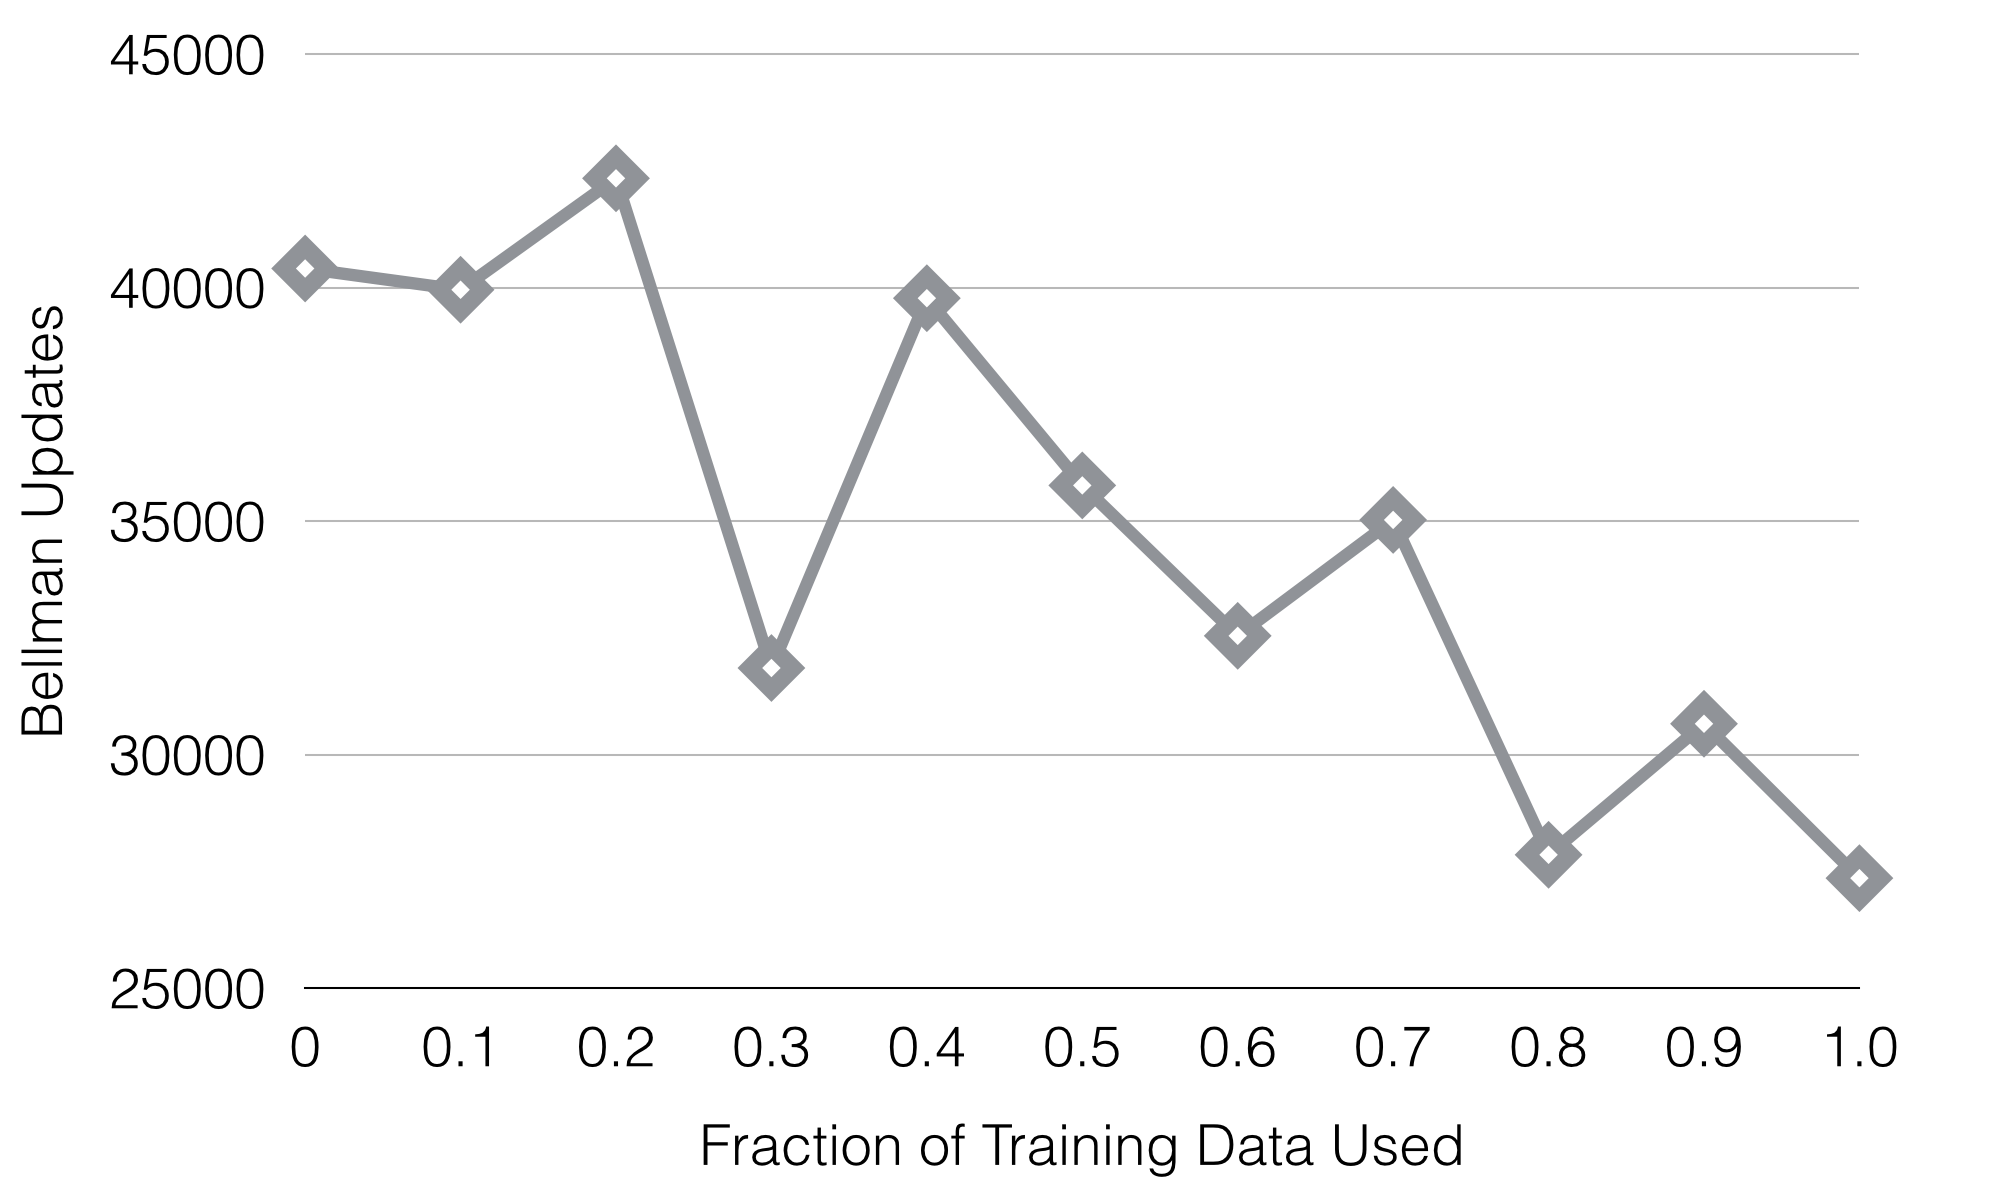
\includegraphics[scale=0.195]{figures/training_results.png}%
  \caption{Place holder for learning rate results}
  \label{fig:training_results}
\end{figure}

% -- Subsection: Temporally Extended Actions --
\subsection{Temporally Extended Actions}

% -- Figure: Temporally Extended Actions Results --
\dnote{These results are no longer accurate (from the previous iteration of math/implementation}
\begin{table}[H]
\centering
\begin{tabular}{ l  || c c c c}
  Augmentation 						&	CPU	&	Reward 	& Bellman \\ \hline
  \texttt{RTDP}  						&	4.86s	&	-4.66		&	4792.0		\\
  \texttt{w/ MA}  						&	21.73s	&	-4.66		&	5255.0		\\
  \texttt{w/ Options}  					&	6.43s	&	-4.66		&	3890.33		\\
  \texttt{w/ Options + MA}  				&	26.10s	&	-4.66		&	5310.0		\\
  \texttt{w/ Affordances}  				& 	3.48s	&	-4.66		&	1907.0		\\
  \texttt{w/ Affordances+MA}  			& 	7.54s	&	-4.66		&	2088.0		\\
  \texttt{w/ Affordances+Options}  		& 	{\bf 3.32s}	&	-4.66		&	{\bf 1829.66}		\\
  \texttt{w/ Affordances+MA+Options}  	& 	-8.45s	&	-4.66		&	2053.66		\\
\end{tabular}
\caption{Affordances vs. Temporally Extended Actions}
\label{table:temp_ext_acts_results}
\end{table}

% -- Subsection: Baxter --
\subsection{Baxter}

% -- Figure: Baxter results/image
\begin{figure}[H]
\centering
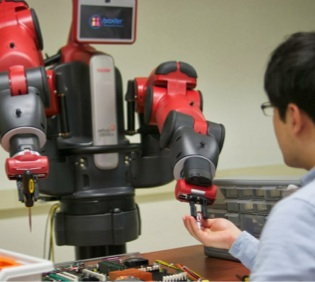
\includegraphics[scale=0.195]{figures/baxter_temp.jpg}%
  \caption{Placeholder for baxter results/image}
  \label{fig:baxter_results}
\end{figure}

% ====== Section: Related Work ======
\section{Related Work}
\label{sec:related-work}

In this section, we discuss the differences between
affordance-aware planning and other forms of knowledge engineering that
have been used to accelerate planning. We divide these approaches
into those that are built to plan in stochastic domains, and those that are
deterministic planners.

% -- Subsection: Stochastic --
\subsection{Stochastic Approaches}

% --- Subsection: Temporally Extended Actions ---
\subsubsection{Temporally Extended Actions}
Temporally extended actions are actions that the agent can
select like any other action of the domain, except executing them
results in multiple primitive actions being executed in
succession. Two common forms of temporally extended actions are {\em
  macro-actions}~\cite{hauskrecht98} ~and {\em options}~\cite{sutton99}. 
Macro-actions are actions that always
execute the same sequence of primitive actions. Options are defined
with high-level policies that accomplish specific sub tasks. For
instance, when an agent is near a door, the agent can engage the
`door-opening-option-policy', which switches from the standard
high-level planner to running a policy that is hand crafted to open
doors. 

Although the classic options framework is not generalizable to different state spaces,
creating {\em portable} options is a topic of active research~\cite{konidaris07,konidaris2009efficient,Ravindran03analgebraic,croonenborghs2008learning,andre2002state,konidaris2012transfer}.

Given the potential for unhelpful temporally extended actions to negatively impact planning time~\cite{Jong:2008zr}, we believe combing affordances with temporally extended actions
may be especially valuable because it will restrict the set of temporally extended actions to those
useful for a task. We conducted a set of experiments to investigate this intuition.

% --- Subsection: Action Pruning ---
\subsubsection{Action Pruning}

Sherstov and Stone~\cite{sherstov2005improving} considered MDPs with a very large 
action set and for which the action set of the optimal policy of a source task could be 
transferred to a new, but similar, target task to reduce the learning time required to find
the optimal policy in the target task. The main difference between our affordance-based 
action set pruning and this action transfer work is that affordances prune away actions on 
a state by state basis, where as the learned action pruning is on per task level. Further, 
with lifted goal descriptions, affordances may be attached to subgoal planning for a significant
benefit in planning tasks where complete subgoal knowledge is known.

Rosman and Ramamoorthy~\cite{rosman2012good} provide a method for learning action
priors over a set of related tasks. Specifically, they compute a Dirichlet distribution over 
actions by extracting the frequency that each action was optimal in each state for each 
previously solved task.

There are a few limitations of the actions priors work that affordance-aware planning
does not possess: (1) the action priors can only be used with planning/learning algorithms
that work well with an $\epsilon$-greedy rollout policy; (2) the priors are only utilized for 
fraction $\epsilon$ of the time steps, which is typically quite small; and (3) as variance in
tasks explored increases, the priors will become more uniform. In contrast, affordance-aware
planning can be used in a wide range of planning algorithms, benefits from the pruned action
set in every time step, and the affordance defined lifted goal-description enables higher-level 
reasoning such as subgoal planning.

% --- Subsubsection: Heuristics ---
\subsubsection{Heuristics}
Heuristics in MDPs are used to convey information about the value of a given state-action pair with respect to the task being solved and typically take the form of either {\em value function initialization},
or {\em reward shaping}. Initializing the value function to an admissible close approximation of the optimal value function has been shown to be effective for LAO* and RTDP~\cite{Hansen:1999qf}.

Reward shaping is an alternative approach to providing heuristics. The planning algorithm uses a modified version of the reward function that returns larger rewards for state-action pairs that are expected to be useful, but does not guarantee convergence to an optimal policy unless certain properties of the shaped reward are satisfied~\cite{potshap}.

A critical difference between heuristics and affordances is that heuristics are highly dependent on the reward function and state space of the task being solved, whereas affordances are state space independent and transferable between different reward functions. However, if a heuristic can be provided, the combination of heuristics and affordances may even more greatly accelerate planning algorithms than either approach alone.

% -- Subsection: Deterministic knowledge engineering approaches --
\subsection{Deterministic Approaches}

There have been several successful attempts at engineering knowledge to
decrease planning time for deterministic planners. These are fundamentally solving
a different problem from what we are interested in, but there approaches are interesting to consider.
\dnote{Need to rephrase this with justification for dealing with deterministic planners}.

% --- Subsubsection: Hierarchical Task Networks ---
\subsubsection{Hierarchical Task Networks}

\dnote{I think we should have a shoutout to Branavan's Learning High Level Plans from Text paper in this section (and include subgoal planning as part of this section}

\enote{I've been writing traditional as I expect we'll discover some HTNs that grapple with the issues stated below -- which we should probably cite}Traditional Hierarchical Task Networks (HTNs) employ \textit{task decompositions} to aid in planning. The goal at hand is decomposed into smaller tasks which are in turn decomposed into smaller tasks. This decomposition continues until primitive tasks that are immediately achievable are derived. The current state of the task decomposition, in turn, informs constraints which reduce the space over which the planner searches.

At a high level both HTNs and affordances fulfill the same role: both achieve action pruning by exploiting some form of supplied knowledge. HTNs do so with the use of information regarding both the task decomposition of the goal at hand and the sorts constraints that said decomposition imposes upon the planner. Similarly, affordances require knowledge as to how to extract values for propositional functions of interest by querying the state.

However there are three of essential distinctions between affordances and traditional HTNs. (1) HTNs deal exclusively with deterministic domains as opposed to the stochastic spaces with which affordances grapple. As a result they produce plans and not policies. (2) Moreover, HTNs do not incorporate reward into their planning. Consequently, they lack mathematical guarantees of optimal planning. \enote{I think.. We should double check this.} (3) On a qualitative level, the degree of supplied knowledge in HTNs surpasses that of affordances: whereas affordances simply require relevant propositional functions, HTNs require not only constraints for sub-tasks but a hierarchical framework of arbitrary complexity. Thus, despite a superficial similarity between affordances and HTNs wherein both employ supplied knowledge, the two deal with disparate forms of planning problems; HTN's planning problem is deterministic, reward-agnostic and necessitates a plethora of knowledge while affordances solve a planning problem that is stochastic, reward-aware and requires only relatively basic knowledge about the domain.
\enote{Need citations for HTNs}
\dnote{needs to be shorter}
% --- Subsubsection: Temporal Logic ---
\subsubsection{Temporal Logic}

Bacchus and Kabanza~\cite{Bacchus95usingtemporal,Bacchus99usingtemporal} provided
planners with domain dependent knowledge in the form of a first-order version of linear
temporal logic (LTL), which they used for control of a forward-chaining planner. With this methodology, 
a \textsc{Strips} style planner may be guided through the search space by checking 
whether candidate plans do not falsify a given knowledge base of LTL formulas, often
achieving polynomial time planning in exponential space.

The primary difference between this body of work and affordance-aware planning is that affordances may be learned (increasing autonomy of the agent), while LTL formulas are far too complicated to learn effectively, placing dependence on an expert.

% ====== Section: Conclusion ======
\section{Conclusion}
\label{sec:conclusion}
\dnote{Conclusion could use some work/rewriting}
We proposed a novel approach to representing transferable knowledge in terms of
{\em affordances}~\cite{gibson77} that allows an agent to efficiently prune actions 
based on domain knowledge, providing a significant reduction in the number of state-action
pairs the agent needs to evaluate in order to act near optimally. We demonstrated the 
effectiveness of the affordance model by comparing standard planners to their affordance-aware
equivalents in a series of challenging planning tasks in the Minecraft domain. Further, we designed
a full learning process that allows an agent to autonomously learn useful affordances that may be used
across a variety of task types, reward functions, and state-spaces, allowing for convenient extensions 
to robotic applications.

We compared the effectiveness of augmenting planners with affordances compared to 
temporally extended actions. The results suggest that affordances, when combined with 
temporally extended actions, provide substantial reduction in the portion of the state-action 
space that needs to be explored.

Lastly, we deployed an affordance-aware planner on a robotic task with a massive 
state space. \dnote{Need to flesh out once we have more detail}.

In the future, we hope to automatically discover useful state-space-specific-subgoals online 
- a topic of some active research \cite{Mcgovern01automaticdiscovery,Simsek:2005:IUS:1102351.1102454}.
This will allow for affordances to plug into high-level subgoal planning, which will reduce the size of the 
explored state-action space and improve the relevance of the action pruning. Additionally, we hope to 
decrease the amount of knowledge given to the planner by implementing lowering the expert seed 
requirements for learning affordances. One plan is to only provide a base of primitive predicates, and 
to implement Incremental Feature Dependency Discovery ~\cite{ICML2011Geramifard_473}, allowing 
our affordance learning algorithm to discover novel preconditions that will further enhance action pruning.
\dnote{Maybe put in a note about the forward search sparse sampling algorithm? Or perhaps the Bayesian planner?}

{\small
\bibliographystyle{plainnat}
\bibliography{main}
}
\end{document}


